\documentclass[border=3mm]{standalone}

\usepackage{tikz}

\begin{document}
	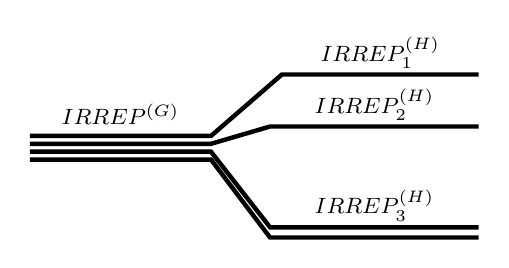
\begin{tikzpicture}
		\draw [ultra thick] (-3.01,-0.29) -- (-0.71,-0.29) node[above,midway] {\footnotesize $IRREP^{(G)}$}-- (0.19,0.49) -- (2.69,0.49) node[midway,above,yshift=-2pt] {\footnotesize $IRREP_1^{(H)}$};
		\draw [ultra thick] (-3.01,-0.39) -- (-0.71,-0.39) -- (0.04,-0.17) -- (2.69,-0.17) node[midway,above,yshift=-2pt] {\footnotesize $IRREP_2^{(H)}$};
		\draw [ultra thick] (-3.01,-0.49) -- (-0.71,-0.49) -- (0.04,-1.45) -- (2.69,-1.45) node[midway,above,yshift=-2pt] {\footnotesize $IRREP_3^{(H)}$};
		\draw [ultra thick] (-3.01,-0.59) -- (-0.71,-0.59) -- (0.04,-1.58) -- (2.69,-1.58);
	\end{tikzpicture}
\end{document}